% SEGMENT OLP-0017-S01
% Part: sets-functions-relations
% Chapter: relations
% Section: graphs

\documentclass[../../../include/open-logic-section]{subfiles}

\begin{document}

\olfileid{sfr}{rel}{grp}
\olsection{கோட்டுருக்கள்}

“கணுக்கள்” அல்லது “முனைகள்” (“முனை” என்பதன் பன்மை) எனப்படும் புள்ளிகள்
விளிம்புகளால் இணைக்கப்பட்டுள்ள ஒரு படம் \emph{கோட்டுரு} ஆகும்.
தனிநிலைக் கணிதத்திலும் கணினி அறிவியலிலும் கோட்டுருக்கள் பரவலாகப்
பயன்படுகின்றன. பல்வேறு வகையான வலையமைப்புகள் போன்ற குறிப்பிட்ட
பொருள்களிலிருந்து, முடிவெடுப்பதால் ஏற்படக்கூடிய விளைவுகள் போன்ற
அருவமான அமைப்புகள் வரை, தொடர்புகளையும் அமைப்புகளையும் குறிக்கவும்
காட்சிப்படுத்தவும் இவை மிகவும் பயனுள்ளவை. ஆய்வு நூல்களில் பல வகையான
கோட்டுருக்கள் உள்ளன. எடுத்துக்காட்டாக, விளிம்புகளுக்குத் திசை உள்ளதா
இல்லையா, குறியடையாளங்கள் உள்ளனவா இல்லையா, ஒரு கணுவிலிருந்து அதே
கணுவுக்கு விளிம்பு இருக்கலாமா, அதே கணுக்களுக்கு இடையில் ஒன்றுக்கு
மேற்பட்ட விளிம்புகள் இருக்கலாமா என்பவற்றைப் பொறுத்து அவை வேறுபடுகின்றன.
\emph{திசை கோட்டுருக்களுக்கும்} தொடர்புகளுக்கும் ஒரு சிறப்பான இணைப்பு
உள்ளது.

% SEGMENT OLP-0017-S02
\begin{defn}[திசை கோட்டுரு]
ஒரு \emph{திசை கோட்டுரு} $G = \tuple{V, E}$ என்பது
\emph{முனைகளின்} கணம் $V$ மற்றும் \emph{விளிம்புகளின்} கணம்
$E \subseteq V^2$ ஆகியவற்றால் ஆனது.
\end{defn}

% SEGMENT OLP-0017-S03
\begin{explain}
நமது வரையறையின்படி, ஒரு கோட்டுரு என்பது ஒரு கணமும் அந்தக் கணத்தின் மீதான
ஒரு தொடர்பும் சேர்ந்ததே. கோட்டுருக்களைப் பற்றிப் பேசும்போது அவை
படங்களாகக் காட்டப்பட வேண்டும் என்று எதிர்பார்ப்பது இயல்பானதே:
$\tuple{v_1, v_2} \in E$ ஆக இருக்கும்போது, அப்போதும் அப்போது மட்டுமே,
$v_1$, $v_2$ என்ற இரு முனைகளை ஓர் அம்பால் இணைத்துக் கோட்டுருவை வரையலாம்.
ஒரு தொடர்புக்கும் ஒரு கோட்டுருவுக்கும் உள்ள ஒரே வேறுபாடு, கோட்டுரு
முனைகளின் கணத்தைத் தனியாகக் குறிப்பிடுகிறது என்பதே; அதாவது ஒரு
கோட்டுருவில் தனித்த முனைகள் இருக்கலாம். முக்கியமான கருத்து என்னவெனில்,
$X$ என்ற கணத்தின் மீதான ஒவ்வொரு தொடர்பு $R$ ஐயும்
$\tuple{X, R}$ என்ற திசை கோட்டுருவாகக் கருதலாம். மறுதலையாக,
$\tuple{V, E}$ என்ற திசை கோட்டுருவை, $V$ என்ற கணம் வெளிப்படையாகக்
குறிப்பிடப்பட்டுள்ள $E \subseteq V^2$ என்ற தொடர்பாகக் கருதலாம்.
\end{explain}

% SEGMENT OLP-0017-S04
\begin{ex}
$V = \{1, 2, 3, 4\}$, $E =
\{\tuple{1,1}, \allowbreak \tuple{1, 2}, \allowbreak \tuple{1, 3},
\allowbreak \tuple{2, 3}\}$ ஆகியவற்றைக் கொண்ட $\tuple{V, E}$
என்ற கோட்டுரு பின்வருமாறு தோன்றும்:
\begin{align*}
& 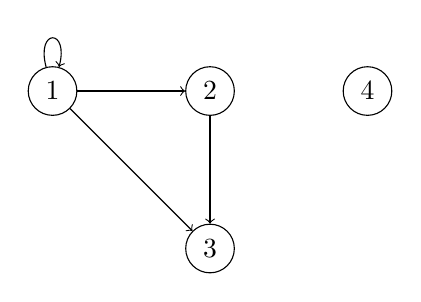
\begin{tikzpicture}[->,node distance=2cm]
  \node[draw,circle] (A) {$1$};
  \node[draw,circle] (B) [right of=A] {$2$};
  \node[draw,circle] (C) [below of=B] {$3$};
  \node[draw,circle] (D) [right of=B] {$4$};
  \draw (A) to [loop above]  (A);
  \draw (A) to  (B);
  \draw (A) to  (C);
  \draw (B) to  (C);
  \end{tikzpicture}
\intertext{இது $\tuple{V', E}$ என்ற கோட்டுருவிலிருந்து வேறுபட்டது;
  அங்கு $V' = \{1, 2, 3\}$. அந்தக் கோட்டுரு பின்வருமாறு தோன்றும்:}
& 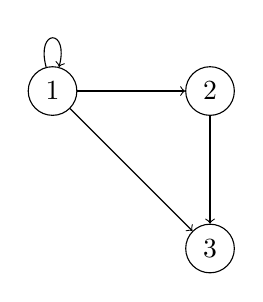
\begin{tikzpicture}[->,node distance=2cm]
  \node[draw,circle] (A) {$1$};
  \node[draw,circle] (B) [right of=A] {$2$};
  \node[draw,circle] (C) [below of=B] {$3$};
  \draw (A) to [loop above]  (A);
  \draw (A) to  (B);
  \draw (A) to  (C);
  \draw (B) to  (C);
  \end{tikzpicture}
\end{align*}
\end{ex}

% SEGMENT OLP-0017-S05
\begin{prob}
  $\{1, 2, 3, 4\}$ என்ற கணத்தின் மீதான, சிறியதாக அல்லது சமமாக இருக்கும்
  தொடர்பு $\le$ ஐ ஒரு கோட்டுருவாகக் கருதி அதற்குரிய படத்தை வரைக.
\end{prob}

\end{document}
